\documentclass[a4paper,norsk,11pt]{interaktiv}

% Importerte pakker
\usepackage{float}
\restylefloat{figure}
\usepackage{ifluatex}
\usepackage{subfigure}
\usepackage{tikz}
\usetikzlibrary{arrows}
\usepackage[parfill]{parskip}    		% Activate to begin paragraphs with an empty line rather than an indent
\usepackage{graphicx}
\usetikzlibrary{snakes}
\usepackage{multicol}

\usepackage[american]{circuitikz}
\ifluatex
  \usepackage{fontspec}
  \setmainfont{Calibri}
  \usepackage{unicode-math}
  \setmathfont{Cambria Math}
\else
  \usepackage[utf8]{inputenc}
\fi

% Underfigurer
\renewcommand{\thesubfigure}{(\arabic{subfigure})}

% Overskrift
\emnekode{TMA4101}
\emnenavn{Matematikk 1 for MTELSYS}
\title{Øving 2 - Følger, rekker og numeriske likningsløsere I}
\author{Frist: 1. sept kl 1400}


% Nye kommandoer
\newcommand{\dee}{\mathop{}\!{d}}

\begin{document}
\pagenumbering{gobble}

\maketitle

I ITGK har du forhåpentligvis lært hvordan man kjører pythonkode, 
og i øvingsopplegget i TMA4101 blir Python en del av hverdagen. 
Lever Pythonoppgaver som en screendump av at du har kjørt koden.

\begin{figure}[htbp]
  \begin{center}
	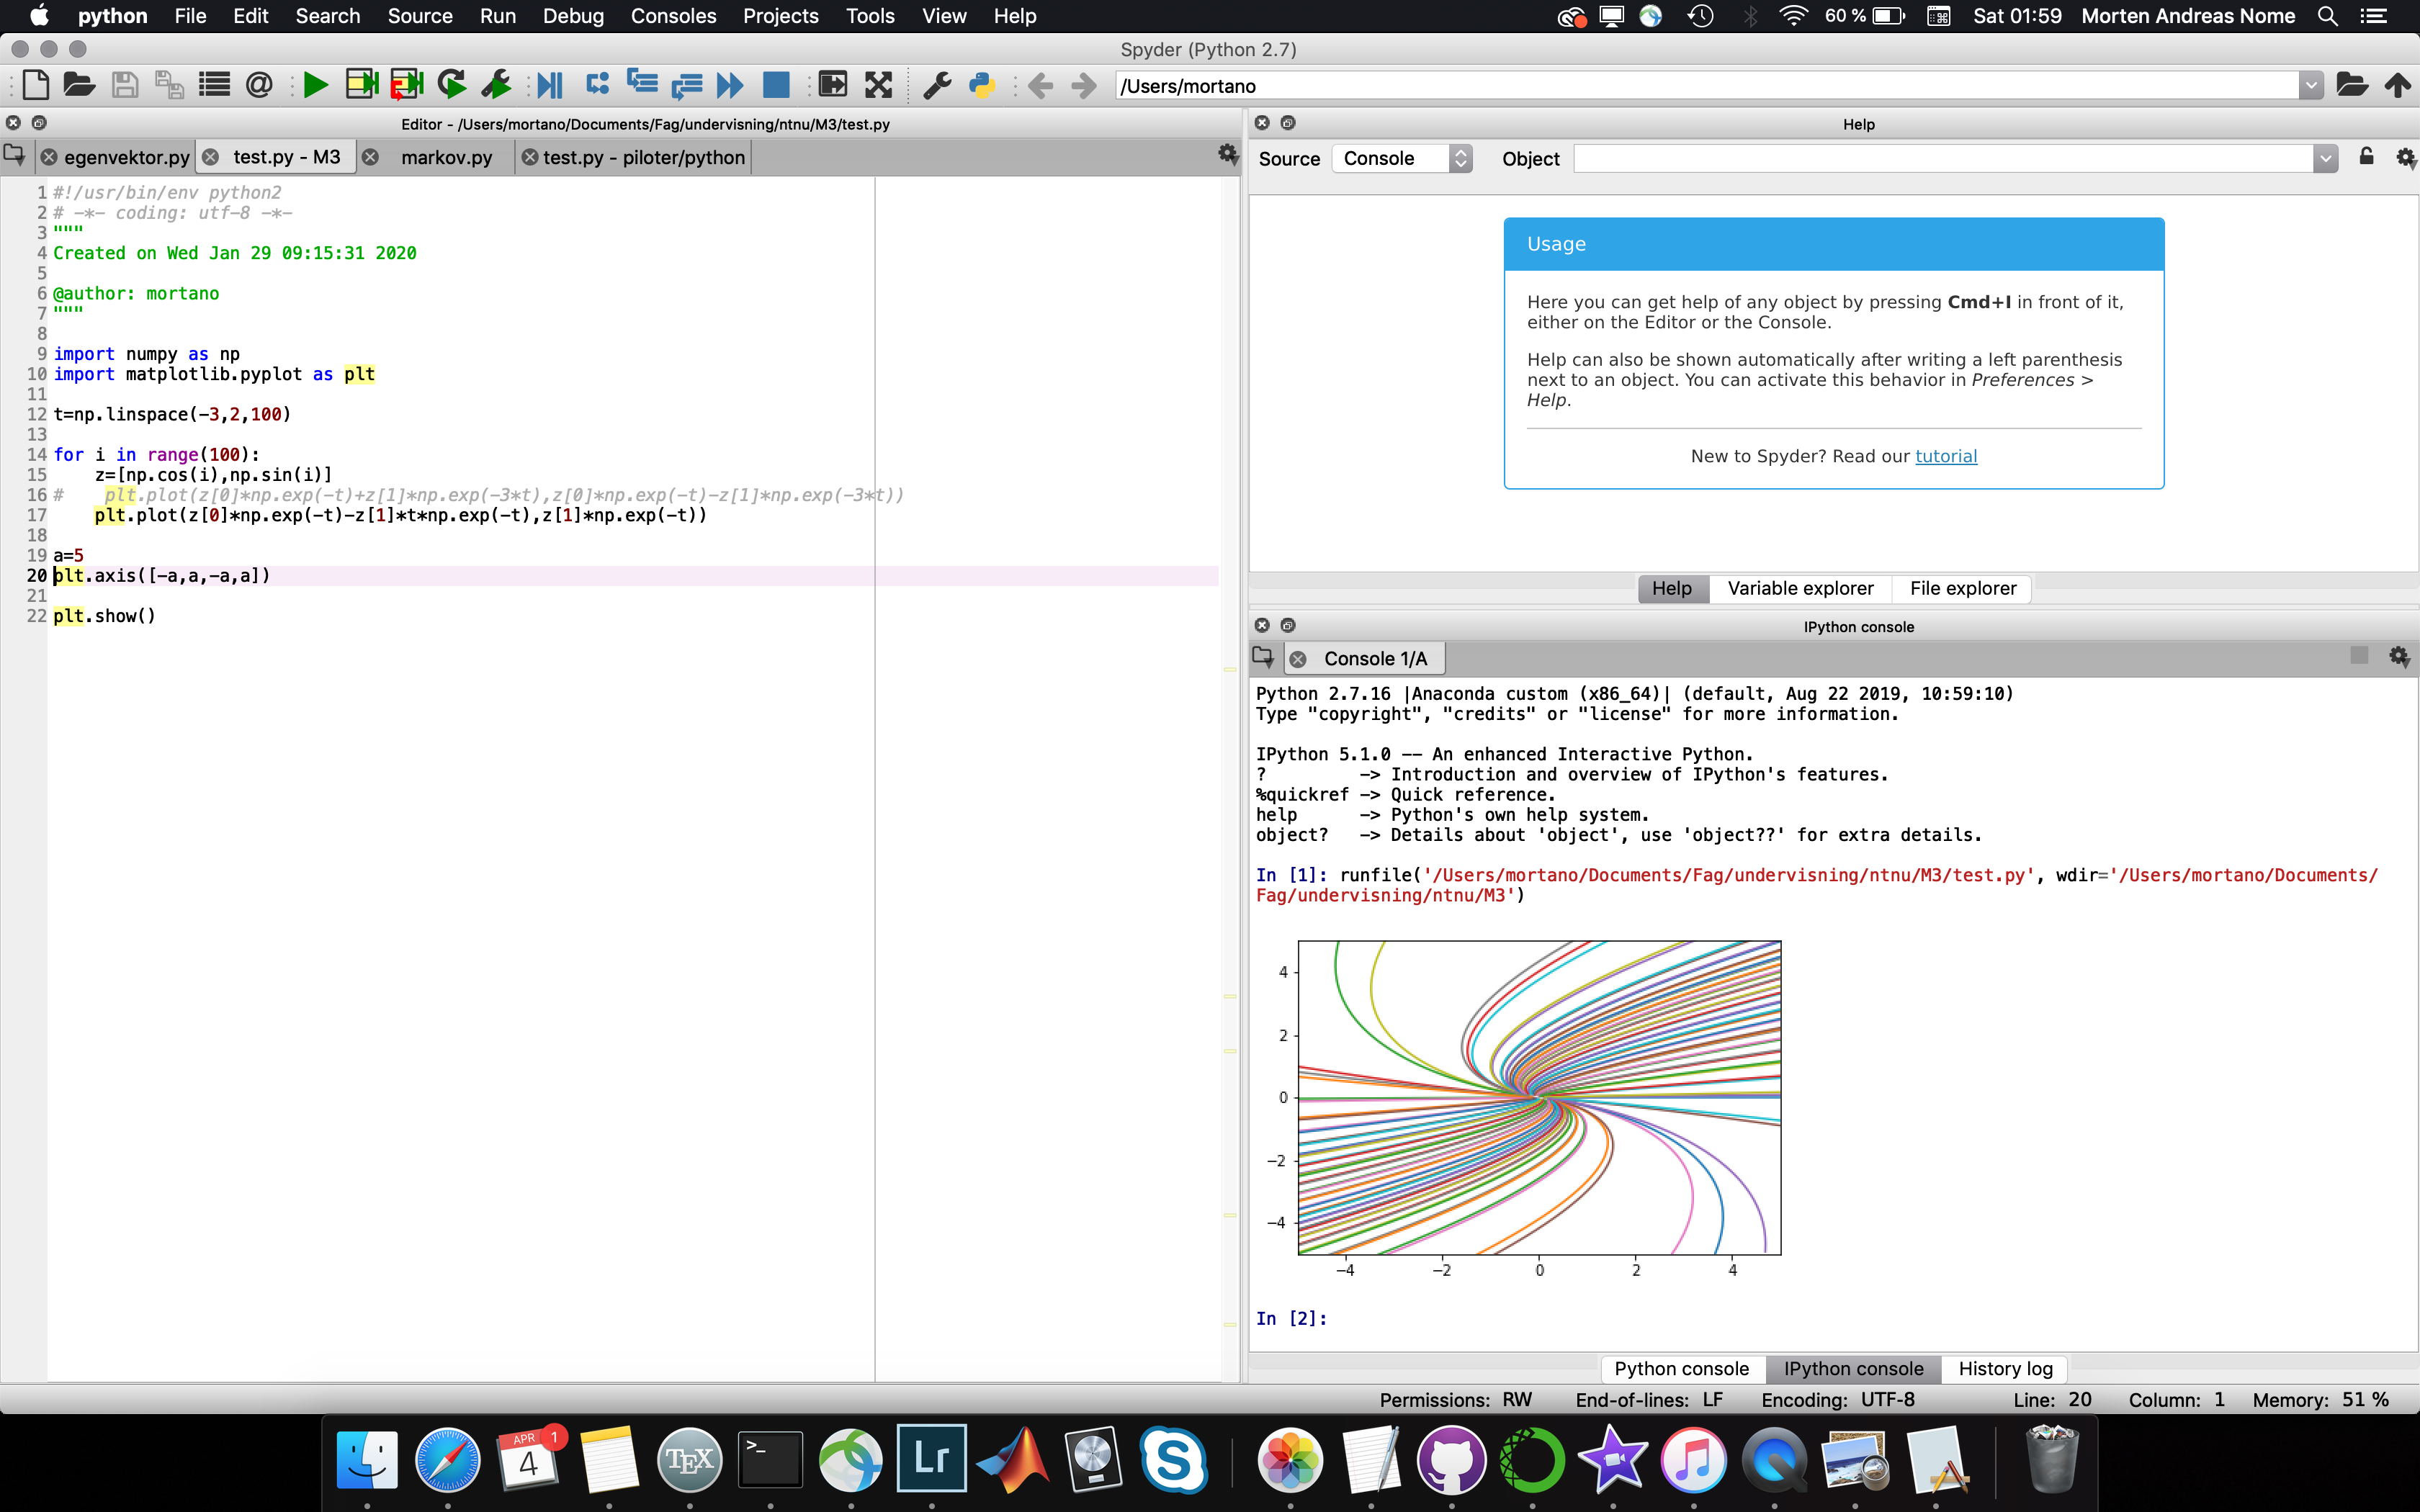
\includegraphics[scale=.27]{screendump.png}
	\label{fig:Num1}
	\end{center}
\end{figure}


\section*{Obligatoriske oppgaver}


\begin{oppgave}{E1}
  La $h$ være vannstanden i et kloakkrør med radius $1$ m, og la $h =
  \cos \theta$.

  \begin{center}
    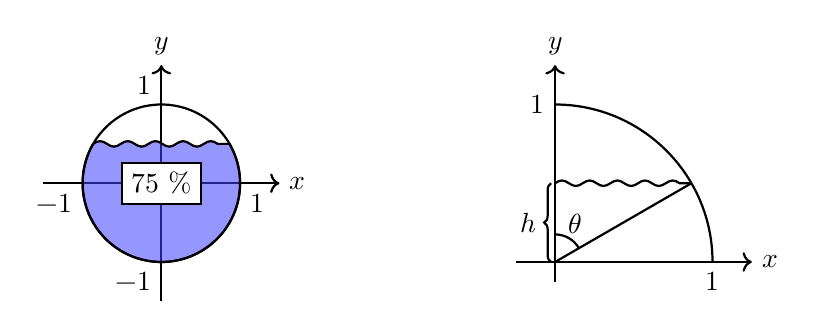
\begin{tikzpicture}[thick]
      \draw[->] (-1.5,0) -- (1.5,0) node[right]{$x$};
      \draw[->] (0,-1.5) -- (0,1.5) node[above]{$y$};
      \filldraw[fill=blue!75!white,fill opacity=0.55] (-0.866,0.5)
        [snake=coil,segment aspect=0,segment amplitude=1pt] --
        (0.866,0.5) arc(30:-210:1cm);
      \draw (0,0) circle (1cm);
      \node[below right] at (1,0){$1$};
      \node[below left] at (-1,0){$-1$};
      \node[above left] at (0,1){$1$};
      \node[below left] at (0,-1){$-1$};
      \node[draw,fill=white,align=center] at (0,0){$75$ \%};

      \begin{scope}[xshift=5cm,yshift=-1cm]
          \draw[->] (-0.5,0) -- (2.5,0) node[right]{$x$};
          \draw[->] (0,-0.25) -- (0,2.5) node[above]{$y$};
          \draw (2,0) arc(0:90:2cm);
          \draw (0,0) -- (2*0.866,1);
          \draw[snake=coil,segment aspect=0,segment amplitude=1pt]
            (0,1) -- (2*0.866,1);
          \draw (0,0.35) arc(90:30:0.35cm)
            node[above,xshift=-0.05cm,yshift=0.05cm]{$\theta$};
          \draw[snake=brace] (-0.05,0) --
            node[left,xshift=-0.05cm]{$h$} (-0.05,1);
          \node[below] at (2,0){$1$};
          \node[left] at (0,2){$1$};
      \end{scope}
    \end{tikzpicture}
  \end{center}

  Når vannet fyller $75$ \% av røret, løser $\theta$
  ligningen
  \begin{equation*}
    2\sin 2\theta + \pi - 4\theta = 0.
  \end{equation*}
Skriv et enkelt pythonscript som bruker Newtons metode eller fikspunktiterasjon til å finne
  vannstanden $h$.
\end{oppgave}

\begin{oppgave}{E2}
Dersom du summerer spenningsfallet over en krets av typen avbildet under, 
vil du få en variant av likningen 
\[
1=i+\ln(i+1).
\]
Denne kan ikke løses analytisk.
Skriv et enkelt pythonscript som finner $v$ med Newtons metode eller fikspunktiterasjon.
\begin{center}
	\begin{circuitikz}
		\draw  (0,1) to [V] (0,3) to [R ] (4,3) to [D] (4,1) to  (0,1);
	\end{circuitikz}
	
%	\begin{circuitikz}
%		\draw (1.1,1) to [short, o-] (0,1) to [R = $R$] (0,4) to[C=$C$] (3,4) to [L = $L$] (3,1) to  [short, -o] (1.9,1);
%		\draw (1.5, 1) node [below] {$v(t)$};
%	\end{circuitikz}
\end{center}
\end{oppgave}


\section*{Anbefalte oppgaver}




\begin{oppgave}{B1} % 75001, 16.12.1994, oppgave 2
  \begin{minipage}[t]{1\textwidth}
  \begin{minipage}[t]{0.5\textwidth}
    Figuren viser de første fem av en uendelig følge av kvadrater.
    Finn summen av omkretsene av alle kvadratene.
  \end{minipage}
  \quad
  \begin{minipage}[t][3cm][b]{0.45\linewidth}
    \centering
    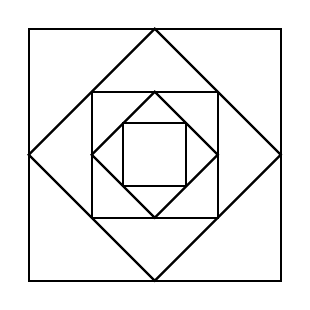
\begin{tikzpicture}[thick,scale=0.8]
      \draw (1.5,1.5) rectangle (2.5,2.5);  
      \draw (2,1) -- (3,2) -- (2,3) -- (1,2) -- cycle;  
      \draw (1,1) rectangle (3,3);
      \draw (2,0) -- (4,2) -- (2,4) -- (0,2) -- cycle;
      \draw (0,0) rectangle (4,4);
    \end{tikzpicture}
  \end{minipage}
\end{minipage}
\end{oppgave}

\begin{oppgave}{C2}
  Anta at en sprettball som slippes rett ned, spretter opp $3/4$ av den
  opprinnelige høyden den ble sluppet fra.  Anta at ballen kun beveger
  seg i vertikal retning.  Hva er avstanden ballen vil bevege seg før
  den blir liggende stille når den slippes fra en høyde på $3$ meter?
\end{oppgave}

Bestem summen til rekkene:

\begin{oppgave}{D3}
    $\quad \displaystyle \sum_{n = 1}^\infty \left(-\frac12\right)^n$
\end{oppgave}

\begin{oppgave}{C4}
    $ \quad \displaystyle \sum_{n = 1}^\infty \frac{2n + 1}{n^2 (n + 1)^2}$.
\end{oppgave}

Avgjør hvorvidt de følgende følgene er begrensede, monotone, og konvergente (og mot hva):


\begin{oppgave}{E5}
\quad $f(n)=\dfrac{n^2 -1}{n}$
\end{oppgave}

\begin{oppgave}{D6}
\quad $f(n)=\dfrac{(n!)^2}{(2n)!} \quad$ (husk at $n! = 1 \cdot 2 \cdot 3 \cdots (n-1) \cdot n$)
\end{oppgave}

\begin{oppgave}{D7}
$
\quad f(n)=\frac{(-1)^n n}{e^n}
$
\end{oppgave}

\begin{oppgave}{C8}
$\quad f(n)=\dfrac{\sin n}{n}$
\end{oppgave}


\begin{oppgave}{B9}
$
\quad  f(n)=(e^{2n}-2n)^{1/n}
$
\end{oppgave}
\setcounter{Punkt}{0}


\begin{oppgave}{A10}
Den rekursive følgen gitt ved $a_1 = 3$ og $a_{n+1} = \sqrt{15 + 2a_n}$ for $n=1,2,3,\ldots$. 
\end{oppgave}

\section*{Relevante eksamensoppgaver fra TMA4100}

\begin{oppgave}{E}
2019H oppgave 1
\end{oppgave}

\section*{Vanskelige oppgaver}

\begin{oppgave}{1}
Bevis regnereglene i teorem 2.8.
\end{oppgave}

\begin{oppgave}{2}
  Vis at når vannet fyller $75$ \% av røret i kloakkoppgaven over, løser $\theta$
  ligningen
  \begin{equation*}
    2\sin 2\theta + \pi - 4\theta = 0.
  \end{equation*}
\end{oppgave}



\end{document}
